\documentclass{llncs}

% \sloppy
% \fussy
\usepackage{microtype}
\usepackage{lmodern}
\usepackage[T1]{fontenc}
%\usepackage{times}
\usepackage{amsmath}
\usepackage{amssymb}
\usepackage{amsfonts}
\usepackage{alltt}
\usepackage{paralist}
\usepackage{soul}
\usepackage{caption}
\usepackage{subcaption}
\usepackage{xspace}
\usepackage{mdwtab}
\usepackage[titletoc,title]{appendix}
\usepackage{multirow}
\usepackage[square,numbers,sort&compress,comma,sectionbib]{natbib}
\usepackage{wrapfig}
\usepackage{algorithm}
\usepackage[noend]{algpseudocode}
\usepackage{tikz}
\usepackage{pgfplots}
\usepackage{hyphenat}
\pgfplotsset{compat=1.12}
\usepackage{hyperref}

\hyphenation{enum-er-at-ive}

% \DeclareCaptionFormat{myformat}{#1#2#3\hrulefill}
% \captionsetup[figure]{format=myformat}

\DeclareCaptionFormat{myformat}{#1#2{\fontsize{8.5}{10}\sffamily\selectfont {#3}}}
\captionsetup[figure]{format=myformat}
\captionsetup[table]{format=myformat}

\newcommand\comment[1]{}
\newcommand\arsays[1]{{\bf AR: #1}}
\newcommand\ausays[1]{{\bf AU: #1}}

\renewcommand\subparagraph[1]{\smallskip\noindent{\em #1.}}
\makeatletter
\newcommand{\@chapapp}{\relax}
\makeatother
\newcommand{\ie}{\emph{i.e.}}
\renewcommand{\bibname}{References}
\newcommand\Integers{\mathbb{Z}}
\newcommand\tuple[1]{\langle #1 \rangle}
\newcommand\True{\mathit{True}}
\newcommand\None{\mathit{None}}
\newcommand\Equiv{\mathit{Eq}}
\newcommand\Points{\mathsf{pts}}
\newcommand\Point{\mathsf{pt}}
\newcommand\Verify{\mathsf{verify}}
\newcommand\CexInput{\mathsf{cexpt}}
\newcommand\Predicates{\mathsf{preds}}
\newcommand\Expr{e}
\newcommand\Pred{p}
\newcommand\Terms{\mathsf{terms}}
\newcommand\Term{t}
\newcommand\Cover{\mathsf{cover}}
\newcommand\Powerset[1]{\mathbf{2}^{#1}}
\newcommand\Spec{\Phi}
\newcommand\Size{K}
\newcommand\Grammar{G}
\newcommand\sem[1]{[\![ #1 ]\!]}
\newcommand\SynthFun{f}
\newcommand\range{\mathsf{range}}
\newcommand\FormalParameters{\mathsf{params}}
\newcommand\Productions{\mathsf{prodn}}
\newcommand\Prob[2]{\mathbb{P}_{#1}(#2)}
\newcommand\NonTerminals{\mathcal{N}}
\newcommand\NonTerminal{N}
\newcommand\StartSymbol{S}
\newcommand\Symbols{\mathsf{symbols}}
\newcommand\Rules{\mathcal{R}}
\newcommand\Rule{R}
\newcommand\Theory{\mathcal{T}}
\newcommand\RewritesTo{\rightarrow}
\newcommand\ITE[3]{\mathtt{if}~#1~\mathtt{then}~#2~\mathtt{else}~#3}

\newcommand\DecisionTree{\mathit{DT}}
\newcommand\DTtoExpr[1]{\mathsf{expr}(#1)}
\newcommand\NodesInternal{V_I}
\newcommand\Nodes{V}
\newcommand\node{v}
\newcommand\NodesLeaf{V_L}
\newcommand\EdgesYes{E_Y}
\newcommand\EdgesNo{E_N}
\newcommand\Edges{E}
\newcommand\Attribute{\mathcal{A}}
\newcommand\Label{\mathcal{L}}
\newcommand{\sygus}{{\sffamily\fontsize{8.5}{10}\selectfont
    SyGuS}\xspace}
\newcommand{\dcsolve}{{\sffamily\fontsize{8.5}{10}\selectfont
    DCSolve}\xspace}
\renewcommand{\paragraph}[1]{\par\noindent\textbf{#1.}}
\newcommand{\itparagraph}[1]{\par\noindent\textit{#1.}}
\newcommand{\esolver}{\textsc{esolver}\xspace}
\newcommand{\sketch}{\textsc{sketch}\xspace}
\newcommand{\pwsolve}{{\sffamily\fontsize{8.5}{10}\selectfont
    PWSolve}\xspace}
\newcommand{\labl}[1]{\mathsf{label}(#1)}

% Make floats and equations behave sensibly
\setlength{\intextsep}{1pt}
\setlength{\textfloatsep}{3pt}
\setlength{\floatsep}{2pt}
\abovedisplayskip=3pt plus 3pt minus 9pt
\abovedisplayshortskip=0pt plus 3pt
\belowdisplayskip=3pt plus 3pt minus 9pt
\belowdisplayshortskip=7pt plus 3pt minus 4pt
\setlength\abovecaptionskip{1pt}
\setlength\belowcaptionskip{1pt}

\begin{document}
% \arsays{TODO:}
% \begin{compactitem}
% \item Change main algo to check for distinctness on points in a
%   straightforward manner
% \item
% \end{compactitem}

% \newpage

\pagestyle{plain}
\title{\texorpdfstring{Scaling Enumerative Program Synthesis\\via
    Divide and Conquer}{Scaling Enumerative Program Synthesis via Divide and Conquer}}
% \author{Rajeev Alur \and Arjun Radhakrishna \and Abhishek Udupa}
\author{}
% \institute{University of Pennsylvania}
\institute{}
\maketitle
\vspace*{-6ex}

\begin{abstract}
  Given a semantic constraint specified by a logical formula, and
  syntactic constraints specified by a context-free grammar, the
  Syntax-Guided Synthesis (\sygus) problem is to find an expression
  that satisfies both the syntactic and semantic constraints.
  An enumerative approach to solve this problem is to systematically
  generate all expressions from the syntactic space with some pruning,
  and has proved to be surprisingly competitive in the newly started
  competition of \sygus solvers.  It performs well on small to medium sized
  benchmarks, produces succinct expressions, and has the ability to
  generalize from input-output examples.  However, its performance
  degrades drastically with the size of the smallest solution. To overcome
  this limitation, in this paper we propose an alternative approach to
  solve \sygus instances.

  The key idea  is to employ a divide-and-conquer approach by
  separately enumerating (a) smaller expressions that are correct on
  subsets of inputs, and (b) predicates on inputs that distinguish these
  subsets.  These smaller expressions and predicates are then combined
  using decision trees to obtain an expression that is correct on all
  inputs.  We view the problem of combining expressions and predicates as
  a multi-label decision tree learning problem. We propose a novel
  technique of associating a probability distribution over the set of
  labels that a sample can be labeled with. This enables us to use
  standard information-gain based heuristics to learn a compact decision
  tree.

  We report a prototype implementation and evaluate it on the benchmarks
  from the \sygus 2015 competition. Our tool is able to match the running
  times and the succinctness of solutions of both standard enumerative
  solver as well as the latest white-box solvers in most cases.  Further,
  our solver is able to solve a large number of instances from the ICFP
  class of benchmarks, which were previously unsolved by all existing
  solvers.
\end{abstract}

\section{Introduction}
\label{sec:intro}

The field of program synthesis relates to automated techniques that
attempt to automatically generate programs from requirements that a
programmer writes.
% Program synthesis is an increasingly popular area of research
% with the introduction of counter-example guided inductive synthesis (CEGIS)
% approach by Solar-Lezama et al, and has been applied to a wide array of
% domains including invariant generation, automated repair of
% programs, binary rewriting, etc~\cite{solar-lezama-05,garg-16}.
It has been applied to various domains such as program
completion~\cite{solar-lezama-05}, program optimization, and automatic
generation of string manipulation programs from input-output
examples~\cite{gulwani-popl-11}, among others.
Recently, Syntax-Guided Synthesis (\sygus) has been proposed as a
back-end exchange format and enabling technology for program
synthesis~\cite{udupa-sygus}.
The aim is to allow experts from different domains to model their
synthesis problems as \sygus instances, and leverage general purpose
\sygus solvers.

In the \sygus approach, a synthesis task is specified using
restrictions on both the form (syntax) and function (semantics) of the
program to be synthesized:
\begin{inparaenum}[(a)]
\item The syntactic restrictions are given in terms of a context-free
  grammar from which a solution program may be drawn.
\item The semantic restrictions are encoded into a specification as an
  SMT formula.
\end{inparaenum}
Most \sygus solvers operate in two cooperating phases: a {\em learning
  phase} in which a candidate program is proposed, and a {\em
verification phase} in which the proposal is checked against the
specification.
\sygus solvers can be broadly categorized into two kinds:
\begin{inparaenum}[(a)]
\item black-box solvers, where the learning phase does not deal with the
  specification directly, but learns from constraints on how a potential
  solution should behave on sample inputs
  points~\cite{udupa-transit,udupa-sygus,saha-15}; and
\item white-box solvers, which attempt learn directly from the
  specification, generally using constraint solving techniques~\cite{reynolds-15,alur-15}.
\end{inparaenum}

% Of the black-box solvers, the most successful, despite its simplicity,
% has been the enumerative solver which won the \sygus competition 2014
% and placed second in \sygus competition 2014.
The enumerative solver~\cite{udupa-sygus}
placed first and second in the \sygus competition 2014 and 2015,
respectively.
It maintains a set of concrete input points, and
in each iteration attempts to produce an expression that is correct on
these concrete inputs.
It does so by enumerating expressions from the grammar and checking if
they are correct on the input points, while pruning away expressions
that behave equivalently to already generated expressions.
If an expression that is correct on the input points is found, it is
verified against the full specification.
If it is incorrect, a counter-example point is found and added to the
set of input points.

Although the enumerative strategy works well when the desired solutions
have small to medium sizes, it does not scale well with the solution
size.  Figure~\ref{figure:random_exponential_graph}
% the x-axis
% represents expression size and the y-axis represents the time taken to
% enumerate all expressions of size up to the expression size.
shows that the time taken to explore all potential solutions
grows exponentially with solution size.  To overcome this scalability issue, we
introduce a divide-and-conquer enumerative algorithm.

The divide-and-conquer enumerative approach is based on this insight:
while the full solution expression to the synthesis problem may be
large, the important individual parts are small.
The individual parts we refer to here are:
\begin{inparaenum}[(a)]
\item {\em terms} which serve as the return value for the solution,
  and
\item {\em predicates} which serve as the conditionals that choose which
  term is the actual return value for a given input.
\end{inparaenum}
For example, in the expression $\ITE{x \leq y}{y}{x}$, the terms are $x$
and $y$, and the predicate is $x \leq y$.
In this example, although the full expression has size $6$,
the individual terms have size $1$ each, and the predicate has size $3$.
Hence, the divide-and-conquer enumerative approach only enumerates terms
and predicates separately and attempts to combine them into a
conditional expression.
% \arsays{Do we need to mention the point-wise/separable restriction here,
% and also the restriction on grammars?}

To combine the different parts of a solution into a conditional
expression, we use the technique of learning decision
trees~\cite{quinlan-86,bishop-book}.  The input points maintained by
the enumerative algorithm serve as the samples, the predicates
enumerated serve as the attributes, and the terms serve as the labels.
A term $\Term$ is a valid label for a point $\Point$ if $\Term$ is
correct for $\Point$.  We use a simple multi-label decision tree
learning algorithm returns a sound decision tree that classifies the
samples soundly, \ie, for each point, following the edges
corresponding to the attribute values (\ie, predicates) leads to a
label (\ie, term) which is correct for the point.

To enhance the quality of the solutions obtained, we extend the basic
divide-and-conquer algorithm to be an \emph{anytime}
algorithm, \ie, the algorithm does not stop when the first
solution is found, and instead continues enumerating terms and
predicates in an attempt to produce more compact
solutions. Decomposing the verification queries into
\emph{branch-level queries} helps in faster convergence.

% \paragraph{Extensions and Optimizations}
% We present two extensions and optimizations to resolve
% various issues that arise in a practical implementation of the
% divide-and-conquer algorithm, as well as to enhance to the quality of
% solutions produced.

% \subparagraph{Anytime extension}
% The anytime extension to the algorithm does not stop when the first
% solution is found, and instead continues enumerating terms and
% predicates in an attempt to produce more compact solutions.
% For example, suppose the synthesizer is attempting to produce a
% conditional equivalent to $x \geq 0 \wedge y \geq 0 \wedge x + y \leq
% 2$.
% Using predicates of size $3$, the most compact solution the synthesizer
% can produce is $y \geq 0 \wedge ((x = 0 \wedge y \leq 2) \vee (x = 1
% \wedge y \leq 1) \vee (x = 2 \wedge y \leq 0))$.
% However, allowing the synthesizer to continue and further enumerate
% predicates of size $4$ lets it to produce the more compact original
% conditional.

% \subparagraph{Decision tree repair}
% During the enumeration process, a term (say $\Term$) which is correct on
% the same set of points as an already generated term (say $\Term'$) is
% discarded.
% However, it may be the case that $\Term$ is correct on a larger set of
% inputs than $\Term'$.
% Hence, if a counter-example is generated when verifying an expression
% $\Expr$ that uses $\Term'$, it might be possible to repair $\Expr$ to
% make it behave correctly on the counter-example by replacing $\Term'$
% with $\Term$.

% \subparagraph{Branch level verification}
% Another more technique we use to generate additional counter-examples
% from a given decision tree is to verify each branch (path from root to
% leaf) separately.
% Each such verification call may return additional counter-examples,
% allowing the procedure to gain more information from a single incorrect
% solution.
% For example, to verify the proposed solution expression $\SynthFun(x, y)
% \equiv \ITE{x \leq y}{1}{0}$: instead of checking if there exists an
% input $(x_0, y_0)$ on which the expression behaves incorrectly, branch
% level verification checks separately if
% \begin{inparaenum}[(a)]
% \item there exists an input satisfying $x \leq y$ on which the
%   expression $1$ behaves incorrectly, and
% \item the exists an input satisfying $\neg x \leq y$ on which the
%   expression $0$ behaves incorrectly.
% \end{inparaenum}

\paragraph{Evaluation}
We implemented the proposed algorithm in a prototype tool and
evaluated it on benchmarks from the \sygus competition 2015, both in
the linear integer arithmetic and the bit-vector domain.  The tool was
able to perform on par or better than existing solvers in the
bit-vector domain, and produced compact solutions. The tool was able
to solve $47$ out of the $50$ problems in the ICFP suite of
benchmarks.  % in less than $1$ hour.  To the best of our knowledge,
no other solver has been able to solve the ICFP benchmarks
satisfactorily.  Further, we also observed that the anytime extension
of the algorithm was able to produce more compact solutions in $22$ of
the $47$ solved benchmarks.  We were able to obtain upto $90\%$
reduction in solution size in some cases.  In the linear integer
arithmetic domain, the tool performed much better than existing
black-box solvers, scaling to larger instances. The algorithm was also
competitive with the white-box solvers for small to medium sized
benchmarks. However, for larger benchmarks, the performance was worse,
and the solution size was slightly larger than those produced by
white-box solvers due to the shortcomings of the decision tree
learning algorithm.

\comment{
\paragraph{Summary}
Overall, this paper presents a divide-and-conquer approach to
enumerative synthesis.
The main contributions are as follows:
\begin{inparaenum}[(a)]
\item The main divide-and-conquer algorithm that enumerates only the
  terms and predicates involved in the final solution and combines them
  using a decision tree learning technique;
\item Several novel extensions and optimizations leading to improved
  quality of solutions and performance; and
\item A prototype tool and experimental evaluation demonstrating the
  scalability of the approach and quality of solutions produced.
\end{inparaenum}
}

\vspace*{-2ex}
\section{Illustrative Example}
\label{sec:example}

\begin{wrapfigure}{r}{0.4\textwidth}
  \vspace*{-3ex}
  \begin{alltt}
  \fontsize{8}{10}\selectfont
S ::= T | if (C) then T else T
T ::= 0 | 1 | x | y | T + T
C ::= T \(\leq\) T | C \(\wedge\) C | \(\neg\) C
\end{alltt}
  \vspace*{-2ex}
  \caption{Grammar for linear integer expressions}
  \label{fig:lia_grammar}
  \vspace*{-1ex}
\end{wrapfigure}
We explain the salient points of our approach with an example.
Consider a synthesis task to generate an expression $\Expr$ such that:
\begin{inparaenum}[(a)]
\item $\Expr$ is generated by the grammar from Figure~\ref{fig:lia_grammar}.
\item $\Expr$ when substituted for $f$, in the specification
  $\Spec$, renders it true, where $\Spec \equiv \forall x, y :
  \SynthFun(x, y) \geq x \wedge \SynthFun(x, y) \geq y \wedge
  (\SynthFun(x,y) = x \vee \SynthFun(x,y) = y)$.
\end{inparaenum}
Note that the specification constrains $\SynthFun(x, y)$ to return
maximum of $x$ and $y$.
Here, the smallest solution expression is $\ITE{x \leq y}{y}{x}$.
% The smallest expression generated by the grammar that satisfies this
% specification is

\paragraph{Basic Enumerative Strategy}
We explain the basic enumerative
algorithm~\cite{udupa-transit} using
Table~\ref{table:enumerative_example}.
The enumerative algorithm maintains a set of input points
$\Points$ (initially empty), and proceeds in rounds.
In each round the algorithm proposes a solution expression which
is correct on all of $\Points$.
If this expression is correct on all inputs (verified by an SMT
solver) the algorithm returns it.
Otherwise, a counter-example input point is added to $\Points$.

\begin{table}[!t]
  \setlength{\doublerulesep}{0.4pt}
  \centering
  \fontsize{8}{10}\selectfont
  \begin{tabular*}{\linewidth}{@{\extracolsep{\fill}}clcc}\\\hlx{hv}
      Round no. & \multicolumn{1}{c}{Enumerated expressions} & Candidate Expression & Point added\\\hlx{hvhv}
      1 & $0$ & $0$ & $\{ x \mapsto 1, y \mapsto 0 \}$ \\\hlx{h}
      2 & $0$, $1$ & $1$ & $\{ x \mapsto 0, y \mapsto 2 \}$ \\\hlx{h}
      3 & $0$, $1$, $x$, $y$, $\ldots$, $x + y$,  & $x+y$ & $\{ x \mapsto 1, y \mapsto 2 \}$ \\\hlx{h}
      \vdots & \vdots & \vdots & \vdots\\\hlx{h}
      $n$ & $0$, \ldots, $\ITE{x \leq y}{y}{x}$  & $\ITE{x \leq y}{y}{x}$ &  \\\hlx{hvv}
  \end{tabular*}
  \vspace{1ex}
  \caption{Example run of the basic enumerative algorithm}
  \label{table:enumerative_example}
  \vspace{-3ex}
\end{table}

The algorithm generates the candidate solution expression by
enumerating expressions generated by the grammar in order of size.
In the first round, the candidate expression proposed is the first
expression generated (the expression $0$) as $\Points$ is empty.
Attempting to verify the correctness of this
expression, yields a counter-example point $\{ x \mapsto 1, y \mapsto
0 \}$.  In the second round, the expression $0$ is incorrect on the
point, and the next expression to be correct on all of $\Points$ (the
expression $1$)
is proposed.  This fails to verify as well, and yields the
counter-example point $\{ x \mapsto 0, y \mapsto 2 \}$. In the third
round, all expressions of size $1$ are incorrect on at least one point
in $\Points$, and the algorithm moves on to enumerate larger
expressions.
% and the algorithm moves to expressions of size $3$
% (there are no expressions of size $2$).
% Here, the algorithm might
% generate the expression $0 + x$.  However, this expression is
% immediately discarded as it is equivalent to the expression $x$ (of
% size $1$) on all $\Points$.
After several rounds, the algorithm eventually generates the expression
$\ITE{x \leq y}{y}{x}$ which the SMT solver verifies to be correct.
Note that to get the correct expression, the algorithm had to generate
a large number (in this case, hundreds of expressions).  In general,
the number of expressions grows exponentially with size.  Thus, the
enumerative solver fails to scale to problems which only admit
solutions representable by large expressions.


\paragraph{Divide and Conquer Enumeration}
In the above example, though the solution is large, the
individual components (terms $x$ and $y$, and predicate $x \leq
y$) are rather small and can be quickly enumerated.
% This difference between the sizes of the constituent terms and
% predicates, and the complete solution only increases for larger
% solutions.
%
The divide-and-conquer approach enumerates terms and predicates
separately, and attempts to combine them into a conditional expression.
We explain this idea using an example (see Table~\ref{table:dq_example}).

Similar to the basic algorithm, the divide-and-conquer algorithm
maintains a set of points $\Points$, and works in rounds.
The first two rounds are similar to the run of the basic algorithm.
% the terms $0$ and $1$ are generated, found to be incorrect, and the
% corresponding points are added to $\Points$.
% As before, in the first round, the term $0$ is generated and found to be
% correct on $\Points$ (which is empty).
% The second round is similar to the second round of the basic
% enumerative algorithm.
In contrast to the basic algorithm, the enumeration stops in the third
round after $0$, $1$, $x$, and $y$ are enumerated -- the terms $1$ and
$y$ are correct on $\{ x \mapsto 1, y \mapsto 0 \}$ and $\{ x \mapsto 0,
y \mapsto 2 \}$, respectively, and thus together ``cover'' all of $\Points$.
Now, to propose an expression, the algorithm starts enumerating
predicates until it finds a sufficient number of predicates to generate
a conditional expression using the previously enumerated terms.
The terms and predicates are combined into conditional expression by
learning decision trees (see Section~\ref{sec:decision_trees}).
The candidate expression proposed in the third round is
$\ITE{1 \leq y}{y}{x}$ and the counter-example generated is
$\{ x \mapsto 2, y \mapsto 0 \}$ (see table).
Proceeding further, in the fourth round, the correct expression is
generated.
Note that this approach only generates $4$ terms and $11$ predicates in
contrast to the basic approach which generates hundreds of
expressions.

\begin{table}[!t]
  \setlength{\doublerulesep}{0.4pt}
  \centering
  \fontsize{8}{10}\selectfont
  \begin{tabular*}{\linewidth}{@{\extracolsep{\fill}}cllcc}\\\hlx{hv}

      \multirow{2}{*}{Round no.} & \multicolumn{1}{c}{Enumerated} & \multicolumn{1}{c}{Enumerated} & Candidate & \multirow{2}{*}{Point added} \\
      & \multicolumn{1}{c}{Terms} & \multicolumn{1}{c}{Predicates} & Expression & \\\hlx{hvhv}
      1 & $0$ & $0$ & $\emptyset$ & $\{ x \mapsto 1, y \mapsto 0 \}$ \\\hlx{hv}
      2 & $0$, $1$ & $1$ & $\emptyset$ &  $\{ x \mapsto 0, y \mapsto 2 \}$ \\\hlx{hv}
      \multirow{2}{*}{3} & \multirow{2}{*}{$0$, $1$, $x$, $y$} & $0 \leq 0$, \ldots $0 \leq y$, & \multirow{2}{*}{$\ITE{1 \leq y}{y}{1}$} & \multirow{2}{*}{$\{ x \mapsto 2, y \mapsto 0 \}$} \\
      & & $1 \leq 0$, \ldots $1 \leq y$ & & \\\hlx{hv}
      4 & $0$, $1$, $x$, $y$ & $0 \leq 0$, \ldots $x \leq y$ & $\ITE{x \leq y}{y}{x}$ & \\\hlx{hvv}
  \end{tabular*}
  \vspace{1ex}
  \caption{Example run of the divide-and-conquer enumerative algorithm}
  \label{table:dq_example}
  \vspace{-2ex}
\end{table}

\vspace*{-1mm}
\section{Problem Statement and Background}
\label{sec:problem}
\vspace*{-1mm}
Let us fix the function to be synthesized $\SynthFun$ and its formal
parameters $\FormalParameters$.
We write $\range(\SynthFun)$ to denote the range of $\SynthFun$.
The term {\em point} denotes a valuation of $\FormalParameters$, i.e., a
point is an input to $\SynthFun$.

\begin{example}
  For the running example in this section, we consider a function to be
  synthesized $\SynthFun$ of type $\Integers \times \Integers \to
  \Integers$ with the formal parameters $\FormalParameters = \{ x, y \}$.
  Points are valuations of $x$ and $y$.
  For example, $\{ x \mapsto 1, y \mapsto 2 \}$ is a point.
\end{example}

\paragraph{Specifications}
SMT formulae have become the standard formalism
for specifying semantic constraints for synthesis.
In this paper, we fix an arbitrary theory $\Theory$ and
denote by $\Theory[\Symbols]$, the set of $\Theory$ terms over the
set of symbols $\Symbols$.
A {\em specification} $\Spec$ is a logical formula in a theory $\Theory$
over standard theory symbols and the function to be synthesized
$\SynthFun$.
An expression $\Expr$ {\em satisfies} $\Spec$ ($\Expr \models \Spec$) if
instantiating the function to be synthesized $\SynthFun$ by $\Expr$
makes $\Spec$ valid.

\begin{example}
  \label{ex:running:spec}
  Continuing the running example, we define a specification $\Spec
  \equiv \forall x, y : \SynthFun(x, y) \geq x \wedge \SynthFun(x, y)
  \geq y \wedge f(x, y) = x \vee f(x, y) = y$.
  The specification states that $\SynthFun$ maps each pair $x$ and $y$
  to a value that is at least as great as each of them and equal to one
  of them, i.e., the maximum of $x$ and $y$.
  % The function that returns the maximum of the two input values is the
  % only possible function that satisfies this specification.
\end{example}

\paragraph{Grammars}
An {\em expression grammar} $\Grammar$ is a tuple $\tuple {
\NonTerminals, \StartSymbol, \Rules }$ where:
\begin{inparaenum}[(a)]
\item the set $\NonTerminals$ is a set of non-terminal symbols,
\item the non-terminal $\StartSymbol \in \NonTerminals$ is the initial non-terminal,
\item $\Rules \subseteq \NonTerminals \times
  \Theory[\NonTerminals \cup \FormalParameters]$ is a finite set
  of rewrite rules that map $\NonTerminals$ to $\Theory$-expressions
  over non-terminals and formal parameters.
\end{inparaenum}
We say that an expression $\Expr$ {\em rewrites to} an incomplete
expression $\Expr'$ (written as $\Expr \RewritesTo_\Grammar \Expr'$) if
there exists a rule $\Rule = (\NonTerminal, \Expr'') \in \Rules$ and
$\Expr'$ is obtained by replacing one occurrence of $\NonTerminal$ in
$\Expr$ by $\Expr''$.
Let $\RewritesTo_\Grammar^*$ be the transitive closure of $\RewritesTo$.
We say that an expression $\Expr \in \Theory[\FormalParameters]$
is {\em generated} by the grammar $\Grammar$ (written as $\Expr \in
\sem{\Grammar}$) if $\StartSymbol \RewritesTo_\Grammar^* \Expr$.
Note that we implicitly assume that all terms generated by the grammar
have the right type, i.e., are of the type $\range(\SynthFun)$.

\begin{example}
  \label{ex:running:grammar}
  For the running example, we choose the following grammar.
  The set of non-terminals is given by $\NonTerminals = \{ \StartSymbol, T, C \}$ with
  the initial non-terminal being $\StartSymbol$.
  The rules of this grammar are $\{ (\StartSymbol, T), (\StartSymbol,
      \ITE{C}{\StartSymbol}{\StartSymbol})
    \} \cup \{ (T, x), (T, y), (T, 1), (T, 0), (T, T + T) \} \cup
        \{ (C, T \leq T), (C, C \wedge C), (C, \neg C) \}$.
  This is the standard linear integer arithmetic grammar used for many
  \sygus problems.
  This grammar is equivalent to the one from
  Figure~\ref{fig:lia_grammar}.
\end{example}

\paragraph{The Syntax-Guided Synthesis Problem}
An instance of the \sygus problem is given by a pair $\tuple { \Spec,
\Grammar }$ of specification and grammar.
An expression $\Expr$ is a solution to the instance if $\Expr \models
\Spec$ and $\Expr \in \sem{\Grammar}$.

\begin{example}
  Continuing the running example, for the specification $\Spec$ from
  Example~\ref{ex:running:spec} and the grammar from
  Example~\ref{ex:running:grammar}, one of the solution expressions is
  given by $\SynthFun(x, y) \equiv \ITE{x \leq y}{y}{x}$.
\end{example}

From our definitions, it is clear that we restrict ourselves to a
version of the \sygus problem where there is exactly one unknown function
to be synthesized, and the grammar does not contain {\tt let} rules.
Further, we assume that our specifications are \emph{point-wise}.
Intuitively, a specification is point-wise, if it only relates an
input point to its output, and not the outputs of different inputs.

Here, we use a simple syntactic notion of point-wise specifications,
which we call \emph{plain separability}, for convenience.
However, our techniques can be generalized to any notion of point-wise
specifications.
Formally, we say that a specification is {\em plainly separable} if can
be rewritten into a conjunctive normal form where each clause is either
\begin{inparaenum}[(a)]
\item a tautology, or
\item every appearing application of the function to be synthesized
  $\SynthFun$ have the same arguments.
\end{inparaenum}

\begin{example}
  The specification for our running example $\Spec \equiv \SynthFun(x,
  y) \geq x \wedge \SynthFun(x, y) \geq y \wedge \SynthFun(x, y) = x
  \vee \SynthFun(x, y) = y$ is plainly separable.
  For example, this implies that the value of $\SynthFun(1, 2)$ can be
  chosen irrespective of the value of $\SynthFun$ on any other point.
  On the other hand, a specification such as $\SynthFun(x, y) = 1
  \Rightarrow \SynthFun(x + 1, y) = 1$ is neither plainly separable nor
  point-wise.
  The value of $\SynthFun(1, 2)$ cannot be chosen independently of the
  value of $\SynthFun(0, 2)$.
\end{example}

The above restrictions make the \sygus problem significantly easier.
However, a large fraction of problems do fall into this class.
% (\arsays{x out of y benchmarks in the \sygus 2015 competition}).
Several previous works address this class of problem (see, for
example, \cite{alur-15,madhusudan-16-pw,reynolds-15}).
% The following example shows that a number of commonly occurring
% specification mores are point-wise specifications.


Simply separable specifications allow us to
define the notion of an expression $\Expr$ satisfying a specification
$\Spec$ on a point $\Point$.
Formally, we say that $\Expr \models \Spec \downharpoonleft
\Point$ if $\Expr$ satisfies the specification obtained by
replacing each clause $C$ in $\Spec$
by $\mathit{Pre}_C(\Point) \Rightarrow C$.
Here, the premise $\mathit{Pre}_C(\Point)$ is given by $\bigwedge_{p \in
\FormalParameters} \mathit{Arg}_C(p) = \Point[p]$ where $\mathit{Arg}_C$ is the
actual argument corresponding to the formal parameter $p$ in the
unique invocation of $\SynthFun$ that occurs in $C$.
We extend this definition to sets of points as follows: $\Expr \models
\Spec \downharpoonleft \Points \Leftrightarrow \bigwedge_{\Point \in
\Points} \Expr \models \Spec\downharpoonleft\Point$.

\begin{example}
  \label{ex:running:correctness_on_point}
  For the specification $\Spec$ of the running example, the function
  given by $\SynthFun(x, y) \equiv x + y$ is correct on the point $\{ x
      \mapsto 0, y \mapsto 3 \}$ and incorrect on the point $\{ x
  \mapsto 1, y \mapsto 2 \}$
\end{example}

\subsection{The Enumerative Solver}
\label{sec:enumeration}

\begin{wrapfigure}{l}{0.46\textwidth}
  \begin{minipage}{0.46\textwidth}
    \begin{algorithm}[H]
      \begin{algorithmic}[1]
        \fontsize{8}{10}\selectfont
        \Require Grammar $\Grammar = \tuple { \NonTerminals, \StartSymbol, \Rules }$
        \Require Specification $\Spec$
        \Ensure $\Expr$ s.t.  $\Expr \in \sem{\Grammar} \wedge \Expr \models \Spec$
        \State $\Points \gets \emptyset$ \label{line:basic:init}
        \While{$\mathtt{true}$}
        \For {$\Expr \in \Call{enumerate}{\Grammar,\Points}$ }\label{line:basic:enumerate}
        \If { $\Expr \not\models \Spec \downharpoonleft  \Points$ } \textbf{continue} \EndIf\label{line:basic:concrete_check}
        \State $\CexInput \gets \Verify(\Expr, \Spec)$ \label{line:basic:verify}
        \If { $\CexInput = \bot$ } \Return $\Expr$ \EndIf \label{line:basic:return}
        \State $\Points \gets \Points \cup \CexInput$ \label{line:basic:continue}
        \EndFor
        \EndWhile
      \end{algorithmic}
      \caption{Enumerative Solver}
      \label{algo:basic}
    \end{algorithm}
  \end{minipage}
\end{wrapfigure}
The principal idea behind the enumerative solver is to enumerate all
expressions from the given syntax with some pruning.
Only expressions that are distinct with respect to a set of concrete
input points are enumerated.

\noindent
The full pseudo-code is given in Algorithm~\ref{algo:basic}.
Initially, the set of points is set to be empty at
line~\ref{line:basic:init}.  In each iteration, the algorithm calls
the \textsc{enumerate} procedure\footnote{Note that \textsc{enumerate} is
a coprocedure.  Unfamiliar readers may assume that each call to \textsc{enumerate}
returns the next expression from an infinite list of
expressions.} which returns the next element from a (possibly infinite)
list of expressions
such that no two expressions in this list evaluate to the same values
at every point $\Point \in \Points$ (line~\ref{line:basic:enumerate}).
Every expression $\Expr$ in this list is then verified, first on the
set of points (line~\ref{line:basic:concrete_check}) and then fully
(line~\ref{line:basic:verify}).  If the expression $\Expr$ is correct,
it is returned (line~\ref{line:basic:return}).  Otherwise, we pick a
counter-example input point (\ie, an input on which $\Expr$ is
incorrect) and add it to the set of points and repeat
(line~\ref{line:basic:continue}). A full description of the
\textsc{enumerate} procedure can be found in
\ref{section:appendix_esolver}.

\begin{theorem}
  \label{thm:basic_enumeration}
  Given a {\upshape\sygus} instance $(\Spec, \Grammar)$ with at least one solution
  expression, Algorithm~\ref{algo:basic} terminates and returns the
  smallest solution expression.
\end{theorem}

\begin{wrapfigure}{l}{0.5\textwidth}
\centering
\begin{tikzpicture}
\begin{semilogyaxis}[
width=5cm,
height=5cm,
xlabel=Expression Size,
ylabel=Time to enumerate (s),
tick align=outside,
grid=both,
xtick = {2, 4, 6, 8, 10},
ytick = {0.0001, 0.01, 1, 100, 10000, 1000000, 10000000}
]
\addplot[mark=*,color=black] table {enumeration.dat};
\end{semilogyaxis}
\end{tikzpicture}
\caption{Scalability of Enumeration}
\label{figure:random_exponential_graph}
\end{wrapfigure}
\paragraph{Features and Limitations}
The algorithm based on enumeration performs surprisingly well, considering its
simplicity, on small to medium sized benchmarks
(see~\cite{udupa-transit,udupa-sygus}).
Further, due to the guarantee of Theorem~\ref{thm:basic_enumeration}
that the enumerative approach produces small solutions, the algorithm is
capable of generalizing from specifications that are input-output
examples.

However, enumeration quickly fails to scale with growing size of
solutions.
Figure~\ref{figure:random_exponential_graph} shows the time taken (in seconds) to
generate all expressions up to a given size for the grammar
from Figure~\ref{fig:lia_grammar}.
As can be seen from the graph, the time taken grows exponentially with
the size.


\vspace*{-2ex}
\section{The Divide-and-Conquer Enumeration Algorithm}
\label{sec:algo}

% We first present some necessary definitions and concepts for the divide
% and conquer enumeration algorithm.

\paragraph{Conditional Expression Grammars}
We introduce conditional expressions grammars that separate an
expression grammar into two grammars that generate:
\begin{inparaenum}[(a)]
\item the return value expression, and
\item the conditionals that decide which return value is chosen.
\end{inparaenum}
These generated return values (terms) and conditionals (predicates) are
combined using if-then-else conditional operators.

A {\em conditional expression grammar} is a pair of grammars $\tuple{
\Grammar_T, \Grammar_P }$ where:
\begin{inparaenum}[(a)]
\item the {\em term grammar} $\Grammar_T$ is an expression grammar
  generating terms of type $\range(\SynthFun)$; and
\item the {\em predicate grammar} $\Grammar_P$ is an expression
  grammar generating boolean terms.
\end{inparaenum}
The set of expressions $\sem{\tuple{ \Grammar_T, \Grammar_P }}$
generated by $\tuple{ G_T, G_P }$ is the smallest set of expressions
$\Theory[\FormalParameters]$ such that:
\begin{inparaenum}[(a)]
\item $\sem{\Grammar_T} \subseteq \sem{\tuple{ \Grammar_T, \Grammar_P
  }}$, and
\item $\Expr_1, \Expr_2 \in \sem{\tuple{ \Grammar_T, \Grammar_P }}
  \wedge \Pred \in \sem{\Grammar_P} \implies
  \ITE{\Pred}{\Expr_1}{\Expr_2} \in \sem{\tuple{ \Grammar_T, \Grammar_P }}$
\end{inparaenum}
Most commonly occurring \sygus grammars in practice can be rewritten
as conditional expression grammars automatically.
% in a straightforward and automated manner.
% However, it is easy to construct a grammar that cannot be decomposed
% into a conditional expression grammar.

\begin{example}
  The grammar from Example~\ref{ex:running:grammar} is easily decomposed
  into a conditional expression grammar $\tuple{\Grammar_T, \Grammar_P}$
  where:
  \begin{inparaenum}[(a)]
  \item the term grammar $\Grammar_T$ contains only the non-terminal
    $T$, and the rules for rewriting $T$.
  \item the predicate grammar $\Grammar_P$ contains the two
    non-terminals $\{ T, C \}$ and the associated rules.
  \end{inparaenum}
\end{example}

\paragraph{Decision Trees}
We use the concept of decision trees from machine learning literature to
model conditional expressions.
Informally, a decision tree $\DecisionTree$ maps {\em samples} to {\em
labels}.
Each internal node in a decision tree contains an {\em attribute} which
may either hold or not for each sample, and each leaf node contains a
label.
In our setting, labels are terms, attributes are predicates, and samples
are points.

To compute the label for a given point, we follow a path from the root
of the decision tree to a leaf, taking the left (resp. right) child at
each internal node if the attribute holds (resp.  does not hold) for the
sample.
The required label is the label at the leaf.
We do not formally define decision trees, but instead refer the reader
to a standard text-book (see, for example,~\cite{bishop-book}).

\begin{example}
  Figure~\ref{fig:dt} contains a decision tree in our setting, i.e.,
  with attributes being predicates and labels being terms.
  To compute the associated label with the point $\Point \equiv \{ x
  \mapsto 2, y \mapsto 0 \}$:
  \begin{inparaenum}[(a)]
  \item we examine the predicate at the root node, i.e., $y \leq 0$ and
    follow the left child as the predicate hold for $\Point$;
  \item examine the predicate at the left child of the root node, i.e,
    $x \leq y$ and follow the right child as it does not hold; and
  \item return the label of the leaf $x + y$.
  \end{inparaenum}
\end{example}
\vspace*{-1ex}

\begin{wrapfigure}{l}{0.33\textwidth}
  \centering
  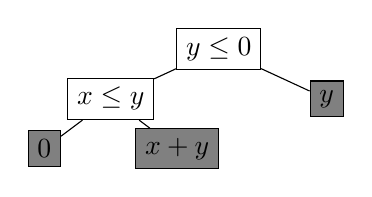
\begin{tikzpicture}
    [every tree node/.style={draw}, level distance=18pt,
      level 1/.style={sibling distance=78pt},
      level 2/.style={sibling distance=48pt},
    level 3/.style={sibling distance=23pt}]
    \node[draw] {$y \leq 0$}
      child {node[draw] {$x \leq y$}
        child {node[fill=gray,draw] {$0$}}
        child {node[fill=gray,draw] {$x + y$}}
      }
      child {node[fill=gray,draw] {$y$}}
      ;
  \end{tikzpicture}
  \vspace*{1pt}
  \caption{Sample decision tree}
  \label{fig:dt}
\end{wrapfigure}
% Every decision tree corresponds to an if-then-else expression.
% with the
% conditionals given by the attributes, and the terms given by the
% labels.
\noindent
The expression $\DTtoExpr{\DecisionTree}$ corresponding to a
decision tree $\DecisionTree$ is defined as:
\begin{inparaenum}[(a)]
\item the label of the root node if the tree is a single leaf node; and
\item
  $\ITE{\Pred}{\DTtoExpr{\DecisionTree_L}}{\DTtoExpr{\DecisionTree_Y}}$
  where $\Pred$ is the attribute of the root node, and $\DecisionTree_L$ and
  $\DecisionTree_Y$ are the left and right children, otherwise.
\end{inparaenum}

\noindent
Decision tree learning is a technique that learns a decision tree from a
given set of samples.
A decision tree learning procedure is given:
\begin{inparaenum}[(a)]
\item a set of samples (points),
\item a set of labels (terms), along with a function that maps a label to the
  subset of samples which it covers; and
\item a set of attributes (predicates).
\end{inparaenum}
A sound decision tree learning algorithm returns a decision tree
$\DecisionTree$ that classifies the points correctly, i.e., for every
sample $\Point$, the label associated with it by the decision tree covers
the point.
We use the notation {\sc LearnDT} to denote a generic, sound
decision tree learning procedure.
The exact procedure we use for decision tree learning in
Section~\ref{sec:decision_trees}.

\vspace*{-2ex}
\subsection{Algorithm}
\label{sec:algo:main}

Algorithm~\ref{algo:main} presents the full divide-and-conquer
enumeration algorithm for synthesis.
Like Algorithm~\ref{algo:basic}, the divide-and-conquer algorithm
maintains a set of points $\Points$, and in each iteration:
\begin{inparaenum}[(a)]
\item computes a candidate solution expression $\Expr$
  (lines~\ref{line:main:start_iter}-\ref{line:main:compute_expr});
\item verifies and returns $\Expr$ if it is correct (lines~\ref{line:main:verify}
  and~\ref{line:main:return}); and
\item otherwise, adds the counter-example point into the set $\Points$
  (line~\ref{line:main:add_point}).
\end{inparaenum}

However, the key differences between Algorithm~\ref{algo:main} and
Algorithm~\ref{algo:basic} are in the way the candidate solution
expression $\Expr$ is generated.
The generation of candidate expressions is accomplished in two
steps.

\paragraph{Term solving}
Instead of searching for a single candidate expression that is correct
on all points in $\Points$, Algorithm~\ref{algo:main} maintains a set of
candidate terms $\Terms$.
We say that a term $\Term$ covers a point $\Point \in \Points$ if $\Term
\models \Spec \downharpoonleft \Point$.
The set of points that a term covers is computed and stored in
$\Cover[\Term]$ (line~\ref{line:main:compute_cover}).
Note that the algorithm does not store terms that cover the same set of
points as already generated terms
(line~\ref{line:main:duplicate_cover}).
When the set of terms $\Terms$ covers all the points in $\Points$, i.e., for
each $\Point \in \Points$, there is at least one term that is correct on
$\Point$, the term enumeration is stopped (while-loop condition in
line~\ref{line:term_solver:while}).

\paragraph{Unification and Decision Tree Learning}
In the next step
(lines~\ref{line:main:unify:start}-\ref{line:main:unify:end}), we
generate a set of predicates $\Predicates$ that will be used as
conditionals to combine the terms from $\Terms$ into if-then-else
expressions.
In each iteration, we attempt to learn a decision tree that correctly
labels each point $\Point \in \Points$ with a term $\Term$ such that
$\Point \in \Cover[\Term]$.
If such a decision tree $\DecisionTree$ exists, the conditional
expression $\DTtoExpr{\DecisionTree}$ is correct on all points, i.e.,
$\DTtoExpr{\DecisionTree} \models \Spec \downharpoonleft \Points$.
If a decision tree does not exist, we generate additional terms and
predicates and retry.

\begin{algorithm}
  \begin{algorithmic}[1]
    \fontsize{8}{10}\selectfont
    \Require Conditional expression grammar $\Grammar = \tuple{ \Grammar_T, \Grammar_P }$
    \Require Specification $\Spec$
    \Ensure Expression $\Expr$ s.t.  $\Expr \in \sem{\Grammar} \wedge \Expr \models \Spec$
    \State $\Points \gets \emptyset$ \label{line:main:init}

    \While {$\mathtt{true}$}
    \State $\Terms \gets \emptyset; \Predicates \gets \emptyset; \Cover \gets \emptyset; \DecisionTree = \bot$ \label{line:main:start_iter}

    \While { $\bigcup_{\Term \in \Terms} \Cover[\Term] \neq \Points$ } \label{line:term_solver:while} \Comment { Term solver }
    \State $\Terms \gets \Terms \cup \Call{NextDistinctTerm}{\Points, \Terms, \Cover$}
    \EndWhile

    \While { $\DecisionTree = \bot$ }\label{line:main:unify:start} \Comment { Unifier }
    \State $\Terms \gets \Terms \cup \Call{NextDistinctTerm}{\Points, \Terms, \Cover$}\label{line:main:more_terms}
    \State $\Predicates \gets \Predicates \cup \Call{enumerate}{\Grammar_P,\Points}$\label{line:main:more_preds}
    \State $\DecisionTree \gets \Call{LearnDT}{\Terms, \Predicates}$ \label{line:main:unify:end}
    \EndWhile

    \State $\Expr \gets \DTtoExpr{\DecisionTree}$; $\CexInput \gets \Verify(\Expr, \Spec)$  \Comment { Verifier } \label{line:main:compute_expr} \label{line:main:verify}
    \If { $\CexInput = \bot$ } \Return $\Expr$ \EndIf \label{line:main:return}
    \State $\Points \gets \Points \cup \CexInput$ \label{line:main:add_point}
    \EndWhile

    \Function{NextDistinctTerm}{$\Points, \Terms, \Cover$}
    \While { $\True$ }
    \State $\Term \gets \Call{enumerate}{\Grammar_T,\Points}; \Cover[\Term] \gets \{ \Point \mid \Point \in \Points \wedge \Term \models \Spec \downharpoonleft \Point \} $\label{line:main:compute_cover}
    \If { $\forall \Term' \in \Terms : \Cover[\Term] \neq
    \Cover[\Term']$ } \Return $\Term$ \EndIf \label{line:main:duplicate_cover}
    \EndWhile
    \EndFunction
  \end{algorithmic}
  \caption{\dcsolve: The divide-and-conquer enumeration algorithm}
  \label{algo:main}
\end{algorithm}

\begin{remark}
  In line~\ref{line:main:more_terms}, we generate additional terms even
  though $\Terms$ is guaranteed to contain terms that cover all points.
  This is required to achieve semi-completeness, i.e., without this, the
  algorithm might not find a solution even if one exists.
  See \ref{sec:app:ex} for an example.
\end{remark}

\begin{theorem}
\vspace*{-1mm}
  Algorithm~\ref{algo:main} is sound for the {\upshape\sygus} problem.
  Further, assuming a sound and complete {\sc LearnDT} procedure, if
  there exists a solution expression, Algorithm~\ref{algo:main} is
  guaranteed to find it.
\vspace*{-1mm}
\end{theorem}
The proof of the above theorem is similar to the proof of soundness and
partial-completeness for the original enumerative solver.
The only additional assumption is that the {\sc LearnDT} decision tree
learning procedure will return a decision tree if one exists.
We present such a procedure in the next section.


\vspace*{-1ex}
\subsection{Decision Tree Learning}
\label{sec:decision_trees}
\vspace*{-1ex}

The standard multi-label decision tree learning algorithm (based on
ID3~\cite{quinlan-86}) is presented in Algorithm~\ref{algo:dt_learning}.
The algorithm first checks if there exists a single label (i.e., term)
$\Term$ that applies to all the points (line~\ref{line:dt:single}).
If so, it returns a decision tree with only a leaf node whose label is
$\Term$ (line~\ref{line:dt:leaf}).
Otherwise, it picks the best predicate $\Pred$ to split on based on some
heuristic (line~\ref{line:dt:pick_pred}).
If no predicates are left, there exists no decision tree, and the
algorithm returns $\bot$ (line~\ref{line:dt:bot}).
Otherwise, it recursively computes the left and right sub-trees for the set of
points on which $\Pred$ holds and does not hold, respectively
(lines~\ref{line:dt:left} and~\ref{line:dt:right}).
The final decision tree is returned as a tree with a root (with
attribute $\Pred$), and positive and negative edges to the roots of the
left and right sub-trees, respectively.

\begin{algorithm}
  \begin{algorithmic}[1]
    \fontsize{8}{10}\selectfont
    \Require $\Points$, $\Terms$, $\Cover$, $\Predicates$
    \Ensure Decision tree $\DecisionTree$
    \If { $\exists \Term : \Points \subseteq \Cover[\Term]$ }\label{line:dt:single}
    \Return $\mathit{LeafNode}[\Label \gets \Term]$ \label{line:dt:leaf}
    \EndIf
    \If {$\Predicates = \emptyset$} \Return $\bot$ \EndIf \label{line:dt:bot}
    \State $\Pred \gets \mbox{Pick predicate from $\Predicates$}$\label{line:dt:pick_pred}
    \State $L \gets \Call{LearnDT}{\{ \Point \mid \Pred[\Point] \},
    \Terms, \Cover, \Predicates \setminus \{ \Pred \} }$\label{line:dt:left}
    \State $R \gets \Call{LearnDT}{\{ \Point \mid \neg \Pred[\Point]
    \}, \Terms, \Cover, \Predicates \setminus \{ \Pred \} }$\label{line:dt:right}
    \State \Return $\mathit{InternalNode}[\Attribute \gets \Pred,  \mathit{left} \gets L , \mathit{right} \gets R ]$
  \end{algorithmic}
  \caption{Learning Decision Trees}
  \label{algo:dt_learning}
\end{algorithm}

\paragraph{Information-gain heuristic}
The choice of the predicate at line~\ref{line:dt:pick_pred} influences
the size of the decision tree learned by
Algorithm~\ref{algo:dt_learning}, and hence, in our setting, the size of
the solution expression generated by Algorithm~\ref{algo:main}.
We use the classical information gain heuristic to pick the predicates.
Informally, the information gain heuristic treats the label as a random
variable, and chooses to split on the attribute knowing whose value
will reveal the most information about the label.
We do not describe all aspects of computing information gain, but
refer the reader to any standard textbook on machine
learning~\cite{bishop-book}.
Given a set of points $\Points' \subseteq \Points$ the entropy
$H(\Points')$ is defined in terms of the probability
$\Prob{\Points'}{label(\Point) = t}$ of a point $\Point \in \Point'$ being
labeled with the term $\Term$ as
\[
H(\Points') = -\sum_{\Term} \Prob{\Points'}{\labl{\Point} = \Term} \cdot \log_2{\Prob{\Points'}{\labl{\Point} = \Term}}
\]
Further, given a predicate $\Pred \in \Predicates$, the information
gain of $\Pred$ is defined as
\[
G(\Pred) = \frac{|\Points_{\mathrm{y}}|}{|\Points|} \cdot
H(\Points_{\mathrm{y}}) + \frac{|\Points_{\mathrm{n}}|}{|\Points|} \cdot
H(\Points_{\mathrm{n}})
\]
where $\Points_{\mathrm{y}} = \{\Point \in \Points \mid \Pred[\Point]\}$ and
$\Points_{\mathrm{n}} = \{\Point \in \Points \mid \neg\Pred[\Point]\}$.
Hence, at line~\ref{line:dt:pick_pred}, we compute the value $G(\Pred)$
for each predicate in $\Predicates$, and pick the one which maximizes
$G(\Pred)$.

We use conditional probabilities $\Prob{\Points'}{\labl{\Point} = \Term \mid
\Point}$ to compute the probability $\Prob{\Points'}{\labl{\Point} = t}$.
The assumption we make about the prior distribution is that the
likelihood of a given point $\Point$ being labeled by a given term
$\Term$ is proportional to the number of points in $\Cover[\Term]$.
Formally, we define:
\[
    \Prob{\Points'}{\labl{\Point} = t \mid \Point} =
    \begin{cases}
        \qquad\qquad\quad 0  & \mathrm{if}\ \Point \notin \Cover[\Term]\\
      \displaystyle
      \frac{\strut\displaystyle\vert \Cover[\Term] \cap \Points' \vert}{\strut\displaystyle\sum_{\Term'
          | \Point \in \Cover[\Term']} \vert \Cover[\Term'] \cap \Points' \vert } & \mathrm{if}\
      \Point \in \Cover[\Term] \\
    \end{cases}
\]
Now, the unconditional probability of an arbitrary point being labeled
with $\Term$ is given by $\Prob{\Points'}{\labl{\Point} = \Term} = \sum_{\Point}
\Prob{\Points'}{\labl{\Point} = \Term \mid \Point}\cdot\Prob{\Points'}{\Point}$.
Assuming a uniform distribution for picking points, we have that
\[
    \Prob{\Points'}{\labl{\Point} = t} =  \frac{1}{\vert \Points \vert} \cdot \sum_{\Point} \Prob{\Points'}{\labl{\Point} = \Term \mid \Point}
\]


\subsection{Extensions and Optimizations}
\label{sec:optimizations}

% We will now discuss several extensions and optimizations for
% Algorithm~\ref{algo:main}.
\paragraph{The Anytime Extension}
Algorithm~\ref{algo:main} stops enumeration of terms and predicates as
soon as it finds a single solution to the synthesis problem.
However, there are cases where due to the lack of sufficiently good
predicates, the decision tree and the resulting solution can be large
(see Example~\ref{ex:continuing}).
Instead, we can let the algorithm continue by generating more
terms and predicates.
This could lead to different, potentially smaller decision trees and
solutions.
% Note that this is in contrast to divide-and-conquer techniques that use
% constraint solving to generate predicates~\cite{alur-15,madhusudan-16-pw}.
% In general, constraint solvers cannot be tuned to give alternate
% solutions.

\begin{example}
  \label{ex:continuing}
  Given the specification $(x \geq 0 \wedge y \geq 0) \Rightarrow
(\SynthFun(x, y) = 1 \Leftrightarrow x + y \leq 2)$ and a run of
Algorithm~\ref{algo:main} where the terms $0$ and $1$ are generated;
the terms fully cover any set of points for this specification.
Over a sequence of iterations the predicates are generated in order
of size.  Now, the predicates generated of size $3$
include $x = 0$, $x = 1$, $x = 2$, $y \leq 2$, $y \leq 1$, and $y \leq
0$.  With these predicates, the decision tree depicted in
Figure~\ref{fig:dt:large} is learned, and the corresponding
conditional expression is correct for the specification.  However, if
the procedure continues to run after the first solution is generated,
predicates of size $4$ are generated.  Among these predicates, the
predicate $x + y \leq 2$ is also generated.  With this additional
predicate, the decision tree in Figure~\ref{fig:dt:small} is
generated, leading to the compact solution $\SynthFun(x, y) \equiv
\mathtt{if}~x + y \leq 2~\mathtt{then}~1~\mathtt{else}~0$.
\end{example}

\begin{wrapfigure}{l}{0.45\textwidth}
  \begin{subfigure}{0.45\textwidth}
    \centering
    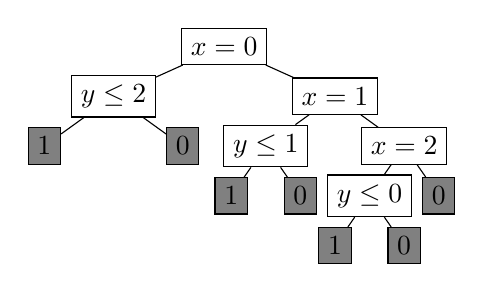
\begin{tikzpicture}
      [every tree node/.style={draw}, level distance=18pt,
      level 1/.style={sibling distance=80pt},
      level 2/.style={sibling distance=50pt},
      level 3/.style={sibling distance=25pt}]
      \node[draw] {$x = 0$}
        child {node[draw] {$y \leq 2$}
          child {node[fill=gray,draw] {$1$}}
          child {node[fill=gray,draw] {$0$}}
        }
        child {node[draw] {$x = 1$}
          child {node[draw] {$y \leq 1$}
            child {node[fill=gray,draw] {$1$}}
            child {node[fill=gray,draw] {$0$}}
          }
          child {node[draw] {$x = 2$}
            child {node[draw] {$y \leq 0$}
              child {node[fill=gray,draw] {$1$}}
              child {node[fill=gray,draw] {$0$}}
            }
            child {node[fill=gray,draw] {$0$}}
          }
        }
        ;
    \end{tikzpicture}
    \caption{Decision tree for predicates of size $3$}
    \label{fig:dt:large}
  \end{subfigure}
  \begin{subfigure}{0.45\textwidth}
    \centering
    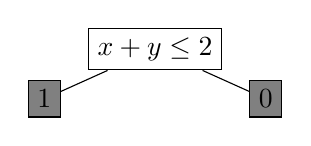
\begin{tikzpicture}
      [every tree node/.style={draw}, level distance=18pt,
      level 1/.style={sibling distance=80pt},
      level 2/.style={sibling distance=50pt},
      level 3/.style={sibling distance=25pt}]

      \node[draw] {$x + y \leq 2$}
        child {node [fill=gray,draw] {$1$}}
        child {node [fill=gray,draw] {$0$}}
      ;
    \end{tikzpicture}
    \caption{Decision tree for predicates of size $4$}
    \label{fig:dt:small}
  \end{subfigure}
  \vspace*{-2ex}
\end{wrapfigure}

\paragraph{Decision Tree Repair}
In Algorithm~\ref{algo:main}, we discard the terms that cover the same
set of points as already generated terms in
line~\ref{line:main:duplicate_cover}.
However, these discarded terms may lead to better solutions than the
already generated ones.

\begin{example}
  \label{ex:dt_repair}
  Consider a run of the algorithm for the running
  example, where the set $\Points$ contains the points $\{ x \mapsto 1,
  y \mapsto 0 \}$ and $\{ x \mapsto -1, y \mapsto 0 \}$.
  Suppose the algorithm first generates the terms $0$ and $1$.
  These terms are each correct on one of the points and are added to
  $\Terms$.
  Next, the algorithm generates the terms $x$ and $y$.
  However, these are not added to $\Terms$ as $x$ (resp. $y$) is correct
  on exactly the same set of points as $1$ (resp. $0$).

  Suppose the algorithm also generates the predicate $x \leq y$ and
  learns the decision tree corresponding to the expression $\Expr \equiv
  \mathtt{if}~x \leq y~\mathtt{then}~0~\mathtt{else}~1$.
  Now, verifying this expression produces a counter-example point, say
  $\{ x \mapsto 1, y \mapsto 2 \}$.
  While the term $0$, and correspondingly, the expression $\Expr$ is
  incorrect on this point, the term $y$ which was discarded as an
  equivalent term to $0$, is correct.
\end{example}

Hence, for a practical implementation of the algorithm we do not discard
these terms and predicates, but store them separately in a map $\Equiv :
\Terms \to \sem{\Grammar_T}$ that maps the terms in
$\Terms$ to an additional set of equivalent terms.
At lines~\ref{line:main:duplicate_cover}, if the check for distinctness
fails, we instead add the term $\Term$ to the $\Equiv$ map.
Now, when the decision tree learning algorithm returns an expression
that fails to verify and returns a counter-example, we attempt to
replace terms and predicates in the decision tree with equivalent ones
from the $\Equiv$ map to make the decision tree behave correctly on the
counter-example.

\begin{example}
  Revisiting Example~\ref{ex:dt_repair}, instead of discarding the terms
  $x$ and $y$, we store them into the $\Equiv$ array, i.e., we set
  $\Equiv(0) = \{ y \}$ and $\Equiv(1) = \{ x \}$.
  Now, when the verification of the expression fails, with the
  counter-example point $\{ x \mapsto 1, y \mapsto 2 \}$, we check the
  term that is returned for the counter-example point--here, $0$.
  Now, we whether any term in $\Equiv(0)$ is correct on the
  counter-example point--here, the term $y$.
  If so, we replace the original term with the equivalent term that is
  additionally correct on the counter-example point and proceed with
  verification.
  Replacing $0$ with $y$ in the expression gives us $\mathtt{if}~x \leq
  y~\mathtt{then}~y~\mathtt{else}~1$.
  Another round of verification and decision tree repair will lead to
  replacing the term $1$ with $x$, giving us the final correct solution.
\end{example}

\paragraph{Branch-wise verification}
In Algorithm~\ref{algo:main}, and in most synthesis techniques, an
incorrect candidate solution is used to generate one counter-example
point.
However, in the case of conditional expressions and point-wise
specifications, each branch (i.e., leaf of the decision tree) can be
verified separately.
Verifying each branch involves rewriting the specification as in the
point-wise verification defined in Section~\ref{sec:problem} -- but
instead of adding a premise to each clause asserting that the arguments
to the function are equal to a point, we add a premise that asserts that
the arguments satisfy all predicates along the path to the leaf.
This gives us two separate advantages:
\begin{compactitem}
\item We are able to generate multiple counter-examples from a single
  incorrect expression.
  This reduces the total number of iterations required, as well as the
  number of calls to the expensive decision tree learning algorithm.
\item It reduces the complexity of each call to the verifier in terms of
  the size of the SMT formula to be checked.
  As verification procedures generally scale exponentially with respect
  to the size of the SMT formula, multiple simpler verification calls
  are often faster than one more complex call.
\end{compactitem}
This optimization works very well along with the decision tree repair
described above as we can verify and repair each branch of the decision
tree separately.

\vspace*{-2mm}
\begin{example}
  Consider the verification of the expression $\ITE{x \leq y}{0}{1}$
  for the running example.
  Instead of running the full expression through the verifier to
  obtain one counter-example point, we can verify the branches
  separately by checking the satisfiability of the formulae $x \leq y
  \wedge f(x, y) = 0 \wedge \neg \Spec$ and $\neg (x \leq y) \wedge f(x,
  y) = 1 \wedge \neg \Spec$.
  This gives us two separate counter-example points.
\end{example}

\vspace{-3ex}
\section{Evaluation}
\label{sec:evaluation}
% \begin{table}[!t]
\centering
\fontsize{8}{10}\selectfont
\begin{tabular*}{\linewidth}{@{\extracolsep{\fill}}lllcccccc}\\\hlx{hv}
\multirow{2}{*}{Benchmark} & Solution & Solution & DT & Max Term & Max Pred & Num \\
& Size & Time (s) & Size &  Size & Size & Points\\\hlx{hv}

icfp\_103\_10 & 33 & 8.9 & 7 & 4 & 6 & 9\\
icfp\_104\_10 & 17 & 0.8 & 5 & 3 & 5 & 6\\
icfp\_105\_1000 & 15 & 24.1 & 5 & 3 & 5 & 4\\
icfp\_105\_100 & 16 & 2.8 & 5 & 3 & 5 & 7\\
icfp\_113\_1000 & 11 & 35.5 & 3 & 4 & 4 & 2\\
icfp\_114\_100 & 20 & 154.6 & 5 & 5 & 5 & 3\\
icfp\_118\_100 & 31 & 13.8 & 7 & 4 & 5 & 4\\
icfp\_118\_10 & 32 & 3.4 & 7 & 4 & 5 & 6\\
icfp\_125\_10 & 57 & 9.6 & 13 & 4 & 6 & 10\\
icfp\_134\_1000 & 33 & 932.3 & 7 & 5 & 6 & 12\\
icfp\_135\_100 & 13 & 34.6 & 3 & 5 & 4 & 2\\
icfp\_139\_10 & 10 & 1.2 & 3 & 4 & 4 & 2\\
icfp\_143\_1000 & 16 & 903.8 & 3 & 5 & 5 & 3\\
icfp\_144\_1000 & 24 & 876.1 & 5 & 5 & 6 & 3\\
icfp\_144\_100 & 36 & 477.8 & 7 & 5 & 6 & 16\\
icfp\_147\_1000 & 12 & 661.8 & 3 & 5 & 4 & 2\\
icfp\_150\_10 & 51 & 1.7 & 11 & 4 & 5 & 6\\
icfp\_21\_1000 & 21 & 302.4 & 5 & 4 & 5 & 5\\
icfp\_25\_1000 & 22 & 92.8 & 5 & 4 & 6 & 8\\
icfp\_28\_10 & 2 & 0.03 & 0 & 2 & 0 & 1\\
icfp\_30\_10 & 14 & 10.2 & 3 & 5 & 4 & 4\\
icfp\_32\_10 & 14 & 8.5 & 3 & 5 & 4 & 2\\
icfp\_38\_10 & 21 & 4.9 & 5 & 4 & 5 & 5\\
icfp\_39\_100 & 12 & 10.6 & 3 & 4 & 5 & 2\\
icfp\_45\_1000 & 9 & 16.9 & 3 & 3 & 4 & 2\\
icfp\_45\_10 & 9 & 0.12 & 3 & 3 & 4 & 2\\
icfp\_5\_1000 & 19 & 44.1 & 5 & 3 & 5 & 4\\
icfp\_51\_10 & 11 & 1.7 & 3 & 4 & 4 & 2\\
icfp\_54\_1000 & 11 & 25.1 & 3 & 4 & 4 & 2\\
icfp\_64\_10 & 21 & 26.7 & 5 & 5 & 5 & 5\\
icfp\_68\_1000 & 26 & 26.9 & 7 & 3 & 5 & 5\\
icfp\_69\_10 & 11 & 1.1 & 3 & 3 & 5 & 5\\
icfp\_7\_1000 & 17 & 61.8 & 5 & 3 & 6 & 9\\
icfp\_7\_10 & 16 & 0.76 & 5 & 3 & 5 & 6\\
icfp\_72\_10 & 13 & 14.4 & 3 & 5 & 4 & 2\\
icfp\_73\_10 & 18 & 0.51 & 5 & 3 & 5 & 3\\
icfp\_81\_1000 & 21 & 382.4 & 5 & 4 & 5 & 7\\
icfp\_82\_100 & 13 & 8.9 & 3 & 3 & 6 & 8\\
icfp\_82\_10 & 13 & 3.5 & 3 & 3 & 6 & 7\\
icfp\_87\_10 & 19 & 5.2 & 5 & 4 & 5 & 5\\
icfp\_93\_1000 & 22 & 127.5 & 5 & 4 & 5 & 9\\
icfp\_94\_1000 & 17 & 29.5 & 5 & 3 & 5 & 4\\
icfp\_94\_100 & 17 & 2.4 & 5 & 3 & 5 & 4\\
icfp\_95\_100 & 220 & 182.5 & 55 & 4 & 7 & 55\\
icfp\_96\_1000 & 49 & 1289.8 & 11 & 5 & 6 & 22\\
icfp\_96\_10 & 57 & 9.5 & 13 & 4 & 6 & 9\\
icfp\_99\_100 & 18 & 201.2 & 5 & 5 & 5 & 4\\
icfp\_14\_1000 & -- & TO & -- & -- & -- & --\\
icfp\_56\_1000 & -- & TO & -- & -- & -- & --\\
icfp\_9\_1000 & -- & TO & -- & -- & -- & --\\\hlx{hv}
\end{tabular*}
\caption{Results on the ICFP benchmark suite, when the algorithm stops
  after discovering the first solution}
\label{table:one_shot_results}
\end{table}

% \begin{table}[!t]
\centering
\fontsize{9}{11}\selectfont
\begin{tabular*}{\linewidth}{@{\extracolsep{\fill}}cllllll}\\\hlx{hv}
\multirow{2}{*}{\# Args} & \multicolumn{3}{c}{D\&Q Enumeration} & \multicolumn{3}{c}{CVC4}\\\hlx{vc{2-4,5-7}v}
& Size & Time (s) & \# Comp. & Size & Time (s) & \# Comp\\\hlx{h}
2 & 6 & $< 0.1$ & 1 & 6 & $< 0.1$ & 1\\
3 & 16 & 0.16 & 3 & 25 & $< 0.1$ & 4\\
4 & 36 & 0.77 & 7 & 55 & $< 0.1$ & 9\\
5 & 76 & 6.2 & 15 & 96 & $< 0.1$ & 16\\
6 & 156 & 63.2 & 31 & 148 & $< 0.1$ & 25\\
7 & 316 & 546 & 63 & 211 & $< 0.1$ & 36\\
8 & -- & TO & -- & 285 & $< 0.1$ & 49\\
9 & -- & TO & -- & 370 & 0.1 & 64\\
10 & -- & TO & -- & 466 & 0.15 & 81\\\hlx{hv}
\end{tabular*}
\vspace*{1mm}
\caption{Results on the parameterized ``max'' benchmarks.}
\label{table:max_results}
\end{table}


We built a prototype \sygus solver that uses the divide-and-conquer
enumerative algorithm.
% based on the ideas presented in this paper.
The tool consists of 3000 lines of Python code implementing the
enumeration, and high-level algorithms and 3000 lines of
C$\raisebox{1pt}{+\!+}$ code implementing the decision tree learning.
% The algorithms for enumeration were implemented in
% about 3000 lines of Python code, while the algorithms for decision
% tree learning were implemented in about 3000 lines of
% C$\raisebox{1pt}{+\!+}$ code.
All experiments were executed on a
32-core machine with four Intel Xeon E7-4820 processors
% running at 2.0 GHz,
and 128 GB of memory, with a one hour time limit.

% \subsection{Goals, Benchmarks and the State-of-the-art}
\paragraph{Goals}
We seek to empirically evaluate how our synthesis algorithm compares
to other state-of-the-art synthesis techniques along the following
dimensions:
\begin{inparaenum}[(a)]
\item
\emph{Performance}: How quickly can the algorithms arrive at a correct
solution?
\item
\emph{Quality}: How \emph{good} are the solutions produced by the
algorithms? We use compactness of solutions
% , in terms of syntactic size,
as a metric for the quality of solutions.
\item
\emph{Effect of continued execution}: How significant is the
improvement in the quality of the solutions generated
% if the algorithm is
given an additional (but fixed) time budget.
\end{inparaenum}

% To compare and contrast the \dcsolve algorithm with contemporary
% techniques along each of these dimensions,
% We did not consider the other classes in the general-track \sygus
% benchmarks because:
% \begin{inparaenum}[(a)]
% \item the solutions were not conditional expressions, or
% \item the benchmarks were not plainly separable, or
% \item the benchmarks were similar to the ones that we considered.
% \end{inparaenum}

\begin{wrapfigure}{l}{0.45\textwidth}%[!t]
\centering
\begin{subfigure}{0.45\textwidth}
  \begin{tikzpicture}
    \fontsize{8}{10}\selectfont
    \begin{axis}[
      width=5cm,
      height=5cm,
      ylabel=\# Benchmarks,
      xlabel=Time (minutes),
      tick align=outside,
      grid=both,
      ytick={0,10,20,30,40,50},
      xtick={0,600,1200,1800,2400,3000,3600},
      xticklabels={0,10,20,30,40,50,60},
      line width=0.7pt
      ]
      \addplot[mark=.,color=black] table {cumulative_completion.dat};
      \addplot[mark=.,color=red] table {cumulative_min_finding.dat};
    \end{axis}
  \end{tikzpicture}
  \caption{Total number of ICFP benchmarks solved by \dcsolve as a
    function of elapsed
    time. Interpretation: The $y$-coordinate of every point on the
    black (resp. red) plot gives the number of benchmarks for which
    the \dcsolve algorithm can produce the first (resp. smallest)
    solution within the time indicated by the $x$-coordinate of the
    point. All times reported here are \emph{per benchmark} times.}
  \label{subfigure:solved_vs_time}
\end{subfigure}
\quad
\begin{subfigure}{0.45\textwidth}
  \begin{tikzpicture}
    \fontsize{8}{10}\selectfont
    \begin{loglogaxis}[
      width=5cm,
      height=5cm,
      xlabel=First Solution Size,
      ylabel=Min. Solution Size,
      tick align=outside,
      grid=major,
      line width=0.7pt,
      ytick={10, 100},
      xtick={10, 100},
      xmin=5,
      ymin=5,
      xmax=230,
      ymax=230
      ]
      \addplot[mark=.,color=gray] table {xequalsy.dat};
      \addplot[only marks,mark=x,color=blue] table {cumulative_improvement.dat};
    \end{loglogaxis}
  \end{tikzpicture}
  \caption{Scatter plot of first vs. minimum size
    solutions. Interpretation: Each point represents a benchmark. The
    $x$-coordinate of each point gives the size of the \emph{first}
    solution produced by \dcsolve. The $y$-coordinate gives the size
    of the \emph{smallest} solution produced by \dcsolve within 3600
    seconds. Points below the $x = y$ line correspond to benchmarks
    which benefit from continued execution, beyond the first solution.}
  \label{subfigure:first_vs_best}
\end{subfigure}
\caption{Summary graphs of experimental results on the ICFP benchmarks}
\vspace*{-6ex}
\end{wrapfigure}
\paragraph{Benchmarks}
We considered two classes of \sygus benchmarks taken from the \sygus
competition 2015.
The first class that we considered consists of the ICFP
benchmarks. These are bit-twiddling problems with
\begin{inparaenum}[(a)]
\item very specific syntactic restrictions on the operations allowed,
  and
\item behavior specified using only concrete input-output examples
\end{inparaenum}
To the best of our knowledge, no existing \sygus solver has been able to
solve these benchmarks. Detailed experimental results on the ICFP
benchmarks can be found in
Tables~\ref{table:anytime_results_1}~and~\ref{table:anytime_results_2}
in \ref{section:appendix_experimental_results}.
% The first column of
% Table~\ref{table:anytime_results} gives the name of the benchmark, the
% second, third, and fourth columns give the size of the first solution
% discovered, the time at which it was discovered by the algorithm, the time taken to discover the solution,
% and the size of the decision tree associated with the solution,
% respectively. The next three columns provide the same details, but for
% the \emph{minimal} sized solution discovered by the
% algorithm.
% Finally, the last column indicates whether the solution
% that was discovered earliest was also the solution with the minimal
% size.

The second class of benchmarks that we considered compute the
maximum of $n$ integers, where $n$ is a
parameter. Detailed results on these benchmarks can be found in
Table~\ref{table:max_results} in \ref{section:appendix_experimental_results}.

\comment{
One can broadly categorize the existing \sygus solvers into two
categories:\begin{inparaenum}[(a)]
\item
\emph{Black-box solvers}, which do not leverage the correctness
specification to guide the search for solutions. Some examples are
\esolver and the stochastic solver~\cite{udupa-sygus}, as well as the
\dcsolve algorithm.
\emph{White-box solvers}, which actively leverage the correctness
specification to generate terms and predicates for solutions. Examples
for white-box solvers include the solvers based on the \textsc{stun}
algorithms~\cite{alur-15}, and the CVC4 solver~\cite{reynolds-15}.
\end{inparaenum}
}

\paragraph{The State-of-the-art}
From empirical observations, black-box algorithms are able to
generalize well from under-constrained correctness specification,
whereas it is not clear how white-box solvers can generalize from such
specifications, given their heavy reliance on the specifications being
complete.  We note that \esolver, which employs an optimized version
of the basic enumerative algorithm discussed earlier won the 2014
\sygus competition and came in second in the 2015 \sygus competition,
losing to the CVC4 solver, which came in first.
\vspace*{-1mm}
\subsection{Discussion}
% We compare the \dcsolve algorithm compares to contemporary
% solvers along the three dimensions described earlier.

\paragraph{Performance}
As
Tables~\ref{table:anytime_results_1}~and~\ref{table:anytime_results_2},
as well as the black plot in Figure~\ref{subfigure:solved_vs_time}
demonstrate, our algorithm was able to produce a solution for 47 out
of the 50 ICFP benchmarks, within an hour.
We emphasize that we know
of no other solver that has been able to provide satisfactory
solutions to these benchmarks.  The solutions produced by our divide
and conquer algorithm, while being compact, are often of size larger
than $20$, indicating that the solutions are beyond the reach of a
basic enumerative strategy.
% Further, as Figure~\ref{figure:random_exponential_graph}
% indicates, it would be impossible to explore expressions of the size
% indicated in Table~\ref{table:anytime_results} --- which are often
% larger than 20 --- using a basic enumeration strategy.
% such as the one used by \esolver.
% The solutions produced by our divide and
% conquer algorithm are quite compact, and
Of the $47$ solved instances, only $5$ benchmarks take longer than $10$
minutes, as seen in Figure~\ref{subfigure:solved_vs_time}.
% of them are computed in less than ten minutes, with only five
% benchmarks taking longer.

Table~\ref{table:max_results} indicates that our algorithm is competitive
with the state-of-the-art CVC4 solver on the parameterized ``max of
$n$ numbers'' benchmarks, for smaller values of $n$. For larger
values of $n$, our algorithm is not as performant. Our investigations
indicated that in the performance drops are largely due to the large
number of concrete counterexample points that the algorithm maintains,
which in turn leads to the decision tree learning algorithms taking
longer.

% To summarize, the \dcsolve algorithm demonstrates vastly better
% performance than other black-box solvers on both benchmark suites, and
% white-box solvers on the ICFP benchmarks.
% For the linear integer arithmetic benchmarks, its performance is
% competitive with white-box solvers.
% while also being able to
% generalize well from input-output examples as we will now discuss.

\paragraph{Quality of Solutions}
For ICFP benchmarks,
Tables~\ref{table:anytime_results_1}~and~\ref{table:anytime_results_2}
indicate that most of the solutions that our algorithm generates are
rather compact, and are of a size that are comprehensible to a
human. We do not know if solutions smaller than these exist. The CVC4
solver has been able to synthesize solutions for some of the ICFP
benchmarks, {\em but only when syntactic restrictions are lifted}. However,
the solutions generated are large case-splits corresponding to the
input-output examples that form the constraints for the problem.
This is because CVC4 is based on model-based quantifier
instantiation, and each input-output example is an instantiation of the
quantifier.
The solutions are extremely large, and are not the intended or desired
solutions.
% We emphasize that no solution generated by our algorithm is a similar large
% conditional expression that matches inputs to outputs.
Our solutions are compact expressions that perform some
computation on the input, to return an output.

In the case of the ``max'' benchmarks, we again see from
Table~\ref{table:max_results} that our algorithm performs well for
small parameter values, often beating the solutions obtained from the
CVC4 solver in terms of size and number of comparisons.
At larger parameter values, the solutions are still reasonably compact
and not excessively large.
The reason for the somewhat larger solutions for
larger parameter values is that the decision tree learning algorithm
is not optimal, \ie, it does not guarantee the most compact decision
tree. Instead a greedy heuristic is used, which rapidly yields
suboptimal solutions as the number of samples (counterexample points)
increases.
% as with the ``max'' benchmarks for larger
% parameter values.
We intend to explore how we can adapt other
heuristics~\cite{madhusudan-16-pw}, into the setting of our problem, in
future work.

\paragraph{Effect of Continued Execution}
For about half the ICFP benchmarks, we were able to obtain a more
compact solution by letting the algorithm continue execution after the
first solution was discovered (last column in
Tables~\ref{table:anytime_results_1}~and~\ref{table:anytime_results_2},
and Figure~\ref{subfigure:first_vs_best}).
Further, the difference in the first and
smallest solutions is sometimes very significant. For example, in the
case of the ``icfp\_95\_100'' benchmark, we see the size of the
solution go down from 220 to 24.
% by almost an order of magnitude, from 220 to 24.
An interesting phenomenon that we observed was that while the size of
the decision tree almost always went down with time, the size of the
solutions sometimes increased.
% our algorithm would
% sometimes find \emph{larger} solutions when allowed to run
% longer.
% However, the size of the decision trees almost always reduced with time.
This is because the algorithm generated larger terms and predicates
over time, increasing the size of the labels and attributes in each node
of the decision tree.

% It turns out that although the decision trees learned were smaller,
% running the algorithm longer also meant that larger terms and predicates
% were enumerated, thus leading to the overall expression sizes of the
% solutions to sometimes increase with time.

Overall, our experimental evaluation suggests that:
% thus allows us to draw the following conclusions:
\begin{inparaenum}[(a)]
\item
The \dcsolve algorithm is able to quickly learn compact solutions,
% for a large fraction of the ICFP benchmarks,
and generalizes well from input-output examples.
\item
The anytime nature of the \dcsolve algorithm is often useful in
reducing the size of the computed solution;
% by allowing additional execution time.
\item
The \dcsolve algorithm works competently on problems from different
classes of benchmarks.
% domaother
% classes of benchmarks that admit conditional expressions as solutions,
% such as the parameterized ``max'' benchmarks.
\end{inparaenum}

\vspace*{-3mm}
\section{Concluding Remarks}
\label{sec:conclusion}
\vspace*{-2mm}

\paragraph{Related Work}
Program synthesis has seen a revived interest in the last decade,
starting from the \sketch
framework~\cite{solar-lezama-05,solar-lezama-06} which
% \sketch uses an
% unoptimized C program as a correctness specification, and a partial
% program with \emph{generator} expressions to specify syntactic
% restrictions, and
proposed the counterexample guided inductive
synthesis (CEGIS). Almost all synthesis
algorithms proposed in recent literature
% --- including the one described in this paper ---
can be viewed as an instantiation of CEGIS.
% More recently, constraint based synthesis approaches
% have been applied to synthesize loop-free programs~\cite{jha-10,
% gulwani-pldi-11}.
Synthesis of string manipulating programs using input-output
examples has found applications in Microsoft's
FlashFill~\cite{gulwani-popl-11}, and the ideas have been generalized
for other domains in a meta-synthesis framework called
FlashMeta~\cite{polozov-15}.
Other recent work in the area of program synthesis have
used type-theoretic approaches~\cite{gvero-13,osera-15,frankle-16} for
program completion and for generating code snippets.
Synthesis of recursive programs and data structure manipulating code
% using constraint solving techniques
% is yet another application of program synthesis that
has also been studied extensively in recent
years~\cite{kuncak-10,kneuss-13,albarghouthi-13,feser-15}.
Lastly, synthesis techniques based on decision trees have been used to
learn program invariants~\cite{garg-16}.

In the area of \sygus, solvers based on enumerative
search~\cite{udupa-transit}, stochastic
search~\cite{schkufza-13,udupa-sygus} and symbolic
search~\cite{gulwani-pldi-11,jha-10} were among the first solvers
developed. The \sketch approach has also been used to develop \sygus
solvers~\cite{jeon-15}. Alchemist~\cite{saha-15} is another solver
that is quite competitive on benchmarks in the linear arithmetic
domains. More recently, white box solvers like the CVC4
solver~\cite{reynolds-15} and the unification based
solver~\cite{alur-15} have also been developed.

The enumerative synthesis algorithm used by
\esolver~\cite{udupa-transit, udupa-sygus} and the work on using decision
trees for piece-wise functions~\cite{madhusudan-16-pw} are perhaps the
most closely related to the work described in this paper.
We have already discussed at length the shortcomings of \esolver that our
algorithm overcomes.
The approach for learning piece-wise functions~\cite{madhusudan-16-pw}
also uses decision trees.
  While the presented framework is generic, the authors instantiate and
  evaluate it only for the linear arithmetic domain with a specific
  grammar.
% \pwsolve presents a generic algorithm which uses decision trees to
% learn a classifier, as well as thresholds for linear
% inequalities.
% Although presented in a generic manner,
% The algorithm has been instantiated only for the domain of linear arithmetic.
% It is unclear how the approach can be instantiated for other
% domains.
  In \dcsolve, neither the decision tree learning algorithm, nor the
  enumeration is domain-specific, making \dcsolve a domain and grammar
  agnostic algorithm.
  The algorithm presented in~\cite{madhusudan-16-pw} can
  easily learn large constants in the linear integer domain.
  This is something that enumerative approaches, including \dcsolve
  struggle to do.
%   Finally, it is unclear how the techniques of~\cite{madhusudan-16-pw}
%   can handle syntactic restrictions in a general manner.
  % whereas
  % \dcsolve can handle syntactic restrictions of any form, being based on
  % enumerative approaches.
 The heuristics used for decision tree learning are different;
  in~\cite{madhusudan-16-pw}, the authors use a heuristic based on
  hitting sets, while we use a information gain heuristic with
  cover-based priors.


\paragraph{Conclusion}
This paper has presented a new enumerative algorithm to solve
instances of the Syntax-Guided Synthesis (\sygus) problem. The
algorithm overcomes the shortcomings of a basic enumerative
algorithm by using enumeration to only learn small expressions which
are correct on subsets of the inputs. These expressions are then used
to form a conditional expression using Boolean combinations of
enumerated predicates using decision trees. We have demonstrated the
ability of the algorithm to generalize from input-output examples by
solving most of the previously unsolved ICFP benchmarks in
the \sygus benchmark suite. The algorithm is generic, efficient,
produces compact solutions,
and is \emph{anytime} --- in that continued execution can potentially
produce more compact solutions.
% than the initially discovered solution.


\bibliographystyle{plainnat}
\setlength{\bibsep}{1pt}
\begin{small}
\bibliography{main}
\end{small}

\newpage
\renewcommand{\thesection}{\appendixname~\Alph{section}}
\begin{appendices}
\section{Detailed Experimental Results for the Anytime Extension}
\label{section:appendix_experimental_results}
\begin{table}
\centering
\fontsize{9}{11}\selectfont
\begin{tabular*}{\linewidth}{@{\extracolsep{\fill}}lllllllc}\\\hlx{hv}
\multicolumn{1}{c}{\multirow{2}{*}{Benchmark}} & \multicolumn{1}{c}{Size} & \multicolumn{1}{c}{Time} & \multicolumn{1}{c}{DT Size} & \multicolumn{1}{c}{Size} & \multicolumn{1}{c}{Time} & \multicolumn{1}{c}{DT Size} & Min\\
& \multicolumn{1}{c}{of first} & \multicolumn{1}{c}{to first} & \multicolumn{1}{c}{for first} & \multicolumn{1}{c}{of min} & \multicolumn{1}{c}{to min} & \multicolumn{1}{c}{for min} & first?\\\hlx{hv}
icfp\_103\_10.sl & 39 & 1.2 & 9 & 23 & 49.3 & 5 & $\times$ \\
icfp\_104\_10.sl & 15 & 0.1 & 5 & 15 & 0.1 & 5 & $\checkmark$ \\
icfp\_105\_1000.sl & 13 & 0.3 & 5 & 13 & 0.3 & 5 & $\checkmark$ \\
icfp\_105\_100.sl & 13 & 0.1 & 5 & 13 & 0.1 & 5 & $\checkmark$ \\
icfp\_113\_1000.sl & 10 & 0.1 & 3 & 10 & 0.1 & 3 & $\checkmark$ \\\hlx{h}
icfp\_114\_100.sl & 18 & 0.7 & 5 & 18 & 0.7 & 5 & $\checkmark$ \\
icfp\_118\_100.sl & 33 & 1.4 & 7 & 15 & 5.9 & 3 & $\times$ \\
icfp\_118\_10.sl & 30 & 0.6 & 7 & 14 & 1.5 & 3 & $\times$ \\
icfp\_125\_10.sl & 18 & 1.3 & 5 & 18 & 1.3 & 5 & $\checkmark$ \\
icfp\_134\_1000.sl & 32 & 3.0 & 7 & 25 & 44.5 & 5 & $\times$ \\\hlx{h}
icfp\_135\_100.sl & 12 & 0.1 & 3 & 12 & 0.1 & 3 & $\checkmark$ \\
icfp\_139\_10.sl & 9 & 0.0 & 3 & 9 & 0.0 & 3 & $\checkmark$ \\
icfp\_14\_1000.sl & 36 & 3.3 & 7 & 18 & 170.8 & 3 & $\times$ \\
icfp\_143\_1000.sl & 15 & 0.5 & 3 & 15 & 0.5 & 3 & $\checkmark$ \\
icfp\_144\_1000.sl & 31 & 5.7 & 7 & 25 & 223.3 & 5 & $\times$ \\\hlx{h}
icfp\_144\_100.sl & 31 & 3.9 & 7 & 24 & 161.8 & 5 & $\times$ \\
icfp\_147\_1000.sl & 11 & 0.1 & 3 & 11 & 0.1 & 3 & $\checkmark$ \\
icfp\_150\_10.sl & 37 & 0.2 & 9 & 22 & 1.1 & 5 & $\times$ \\
icfp\_21\_1000.sl & 18 & 0.4 & 5 & 18 & 0.4 & 5 & $\checkmark$ \\
icfp\_25\_1000.sl & 28 & 1.8 & 7 & 21 & 34.0 & 5 & $\times$ \\\hlx{h}
icfp\_28\_10.sl & 2 & 0.0 & 0 & 2 & 0.0 & 0 & $\checkmark$ \\
icfp\_30\_10.sl & 13 & 0.2 & 3 & 13 & 0.2 & 3 & $\checkmark$ \\
icfp\_32\_10.sl & 13 & 0.1 & 3 & 13 & 0.1 & 3 & $\checkmark$ \\
icfp\_38\_10.sl & 17 & 0.1 & 5 & 13 & 3.9 & 3 & $\times$ \\
icfp\_39\_100.sl & 11 & 0.1 & 3 & 11 & 0.1 & 3 & $\checkmark$ \\\hlx{h}
\end{tabular*}
\vspace*{1mm}
\caption{Results on the ICFP benchmark suite. All times are in seconds.}
\label{table:anytime_results_1}
\end{table}

\begin{table}[!t]
\vspace*{-1ex}
\centering
\fontsize{9}{11}\selectfont
\begin{tabular*}{\linewidth}{@{\extracolsep{\fill}}lllllllc}\\\hlx{hv}
\multicolumn{1}{c}{\multirow{2}{*}{Benchmark}} & \multicolumn{1}{c}{Size} & \multicolumn{1}{c}{Time} & \multicolumn{1}{c}{DT Size} & \multicolumn{1}{c}{Size} & \multicolumn{1}{c}{Time} & \multicolumn{1}{c}{DT Size} & Min\\
& \multicolumn{1}{c}{of first} & \multicolumn{1}{c}{to first} & \multicolumn{1}{c}{for first} & \multicolumn{1}{c}{of min} & \multicolumn{1}{c}{to min} & \multicolumn{1}{c}{for min} & first?\\\hlx{hv}
icfp\_45\_1000 & 9 & 15.6 & 3 & 9 & 15.6 & 3 & $\checkmark$\\
icfp\_45\_10 & 9 & 0.3 & 3 & 9 & 0.3 & 3 & $\checkmark$\\
icfp\_5\_1000 & 19 & 37.4 & 5 & 18 & 2534.9 & 5 & $\times$\\
icfp\_51\_10 & 11 & 1.9 & 3 & 11 & 1.9 & 3 & $\checkmark$\\
icfp\_54\_1000 & 11 & 38.1 & 3 & 11 & 38.1 & 3 & $\checkmark$\\\hlx{h}
icfp\_56\_1000 & -- & TO & -- & -- & TO & -- & -- \\
icfp\_64\_10 & 21 & 21.4 & 5 & 21 & 21.4 & 5 & $\checkmark$\\
icfp\_68\_1000 & 26 & 40.1 & 7 & 26 & 40.1 & 7 & $\checkmark$\\
icfp\_69\_10 & 11 & 1.1 & 3 & 11 & 1.1 & 3 & $\checkmark$\\
icfp\_7\_1000 & 17 & 95.3 & 5 & 17 & 95.3 & 5 & $\checkmark$\\\hlx{h}
icfp\_7\_10 & 16 & 0.7 & 5 & 16 & 0.7 & 5 & $\checkmark$\\
icfp\_72\_10 & 13 & 18.9 & 3 & 13 & 18.9 & 3 & $\checkmark$\\
icfp\_73\_10 & 18 & 0.52 & 5 & 13 & 39.6 & 3 & $\times$\\
icfp\_81\_1000 & 21 & 526.3 & 5 & 17 & 3008.6 & 3 & $\times$\\
icfp\_82\_100 & 13 & 9.7 & 3 & 13 & 9.7 & 3 & $\checkmark$\\\hlx{h}
icfp\_82\_10 & 13 & 3.9 & 3 & 13 & 3.9 & 3 & $\checkmark$\\
icfp\_87\_10 & 19 & 5.2 & 5 & 19 & 5.2 & 5 & $\checkmark$\\
icfp\_9\_1000 & -- & TO & -- & -- & TO & -- & -- \\
icfp\_93\_1000 & 22 & 182.1 & 5 & 21 & 318.9 & 5 & $\times$\\
icfp\_94\_1000 & 17 & 46.8 & 5 & 17 & 46.8 & 5 & $\checkmark$\\\hlx{h}
icfp\_94\_100 & 17 & 2.4 & 5 & 13 & 498.7 & 3 & $\times$\\
icfp\_95\_100 & 220 & 270.8 & 55 & 24 & 330.2 & 7 & $\times$\\
icfp\_96\_1000 & 49 & 2162.3 & 11 & 47 & 2984.1 & 11 & $\times$\\
icfp\_96\_10 & 57 & 12.4 & 13 & 29 & 12.6 & 7 & $\times$\\
icfp\_99\_100 & 18 & 321.9 & 5 & 18 & 321.9 & 5 & $\checkmark$\\\hlx{h}
\end{tabular*}
\vspace*{1mm}
\caption{Results on the ICFP benchmark suite (continued from Table~\ref{table:anytime_results_1}) . All times are in seconds.}
\label{table:anytime_results_2}
\end{table}

% \begin{table}[!t]
\centering
\fontsize{9}{11}\selectfont
\begin{tabular*}{\linewidth}{@{\extracolsep{\fill}}cllllll}\\\hlx{hv}
\multirow{2}{*}{\# Args} & \multicolumn{3}{c}{D\&Q Enumeration} & \multicolumn{3}{c}{CVC4}\\\hlx{vc{2-4,5-7}v}
& Size & Time (s) & \# Comp. & Size & Time (s) & \# Comp\\\hlx{h}
2 & 6 & $< 0.1$ & 1 & 6 & $< 0.1$ & 1\\
3 & 16 & 0.16 & 3 & 25 & $< 0.1$ & 4\\
4 & 36 & 0.77 & 7 & 55 & $< 0.1$ & 9\\
5 & 76 & 6.2 & 15 & 96 & $< 0.1$ & 16\\
6 & 156 & 63.2 & 31 & 148 & $< 0.1$ & 25\\
7 & 316 & 546 & 63 & 211 & $< 0.1$ & 36\\
8 & -- & TO & -- & 285 & $< 0.1$ & 49\\
9 & -- & TO & -- & 370 & 0.1 & 64\\
10 & -- & TO & -- & 466 & 0.15 & 81\\\hlx{hv}
\end{tabular*}
\vspace*{1mm}
\caption{Results on the parameterized ``max'' benchmarks.}
\label{table:max_results}
\end{table}


\vspace*{-1ex}
Detailed results of running our solver on the ICFP benchmarks are
presented in in
Tables~\ref{table:anytime_results_1}~and~\ref{table:anytime_results_2}. For
each benchmark,
we report
\begin{inparaenum}[(a)]
\item the size of the first solution discovered, the time at which it
was discovered, and the associated decision tree size;
\item the same details for the minimal solution discovered; and
\item whether the first solution discovered was itself minimal sized
  solution.
\end{inparaenum}

\comment{
Table~\ref{table:max_results} demonstrates how our algorithm stacks up
against the state-of-the-art CVC4 solver, when evaluated with the
``max'' benchmarks, which are described in Section~\ref{sec:evaluation}.
The columns indicate the sizes of solutions generated, the time to arrive
at the solution, as well as the number of comparisons in the solution
obtained by each of the solvers, for different values of the parameter
$n$, indicated in the first column.
}

\section{Description of the Enumeration Procedure}
\label{section:appendix_esolver}
\begin{algorithm}
  \begin{algorithmic}[1]
    \fontsize{8}{10}\selectfont
    \Require Grammar $\Grammar = \tuple { \NonTerminals, \StartSymbol, \Rules }$ and a set of points $\Points$
    \Ensure Expressions $\tuple { \Expr_1, \Expr_2, \ldots }$ s.t. $\forall i < j : \vert \Expr_i \vert \leq \vert \Expr_j
    \vert \wedge \exists \Point \in \Points : \Expr_i[\Point] \neq \Expr_j[\Point]$
    \ForAll {$\NonTerminal \in \NonTerminals$} $\Productions[\NonTerminals] \gets \emptyset$ \EndFor
    \ForAll {$(\NonTerminal, \Expr) \in \Rules$}\label{line:enumerate:level_one_iter}
    \If { $\Expr \in \Theory[\FormalParameters]$ }
    $\Productions[\NonTerminal] \gets \Productions[\NonTerminal] \cup \{ \Expr \}$  \label{line:enumerate:level_one}
    \EndIf
    \EndFor
    \State $ \Size \gets 1 $
    \While { $\True$ }
    \ForAll {$(\NonTerminal, \Expr) \in \Rules$}
    \State $(\NonTerminal_1, \ldots, \NonTerminal_n) \gets \mbox{List of non-terminals occurring in $\Expr$ }$
    \ForAll { $(\Expr_1, \ldots, \Expr_n) \in \Productions[\NonTerminal_1] \times \cdots \times \Productions[\NonTerminal_n]$ }
    \State $\Expr^* \gets \Expr[\Expr_1/\NonTerminal_1,\ldots,\NonTerminal_n/\Expr_n]$
    \If { $\vert \Expr^* \vert \leq \Size \wedge \forall \Expr' \in
      \Productions[\NonTerminal] . \exists \Point \in \Points :
    \Expr'[\Point] \neq \Expr^*[\Point] $ }
    \State $\Productions[\NonTerminal] \gets \Productions[\NonTerminal] \cup \Expr^*$
    \If { $\NonTerminal = \StartSymbol$ } \textbf{yield} $\Expr^*$ \EndIf
    \EndIf
    \EndFor
    \EndFor
    \State $\Size \gets \Size + 1$
    \EndWhile
  \end{algorithmic}
  \caption{Enumerating distinct expressions from a grammar}
  \label{algo:enumerate}
\end{algorithm}

Algorithm~\ref{algo:enumerate} describes the \textsc{enumerate}
algorithm referred to in Section~\ref{sec:enumeration}. We continue to
use the same notation here that was introduced in Section~\ref{sec:enumeration}.
The \textsc{enumerate} procedure maintains a map $\Productions : \NonTerminals \to
\Powerset{\Theory[\FormalParameters]}$ from non-terminals to
expressions they can produce.
The invariant maintained by the procedure is that every pair of
expressions in $\Productions[\NonTerminal]$ is distinct on $\Points$.

The algorithm starts by first accumulating into
$\Productions[\NonTerminal]$ the expressions that can be produced from
$\NonTerminal$ in one step
(lines~\ref{line:enumerate:level_one_iter}-\ref{line:enumerate:level_one}).
Then, for each possible expression size $\Size$, it attempts to
instantiate each production rule in the grammar with expressions already
generated and stored in $\Productions$, to generate new expressions of
size at most $\Size$.
These newly generated expression are checked for distinctness from
already generated ones, and if so, added to
$\Productions[\NonTerminal]$.
The algorithm returns all the expressions produced from the starting
non-terminal $\StartSymbol$.

\section{Algorithm~\ref{algo:main} without line~\ref{line:main:more_terms}}
\label{sec:app:ex}

Consider the conditional expression grammar given in
Figure~\ref{fig:bad_grammar} and the specification $f(x) = x$.
Note that the grammar can generate terms equivalent to $ax + b$ where
$a, b \geq 0$ and predicates $ax + b < 0$.
The solution expression is obviously $f(x) \equiv x$.


Now, in the first round, the algorithm enumerates the first term, i.e.,
$0$.
Say counter-example point returned is $\Point_1 = \{ x \mapsto 1 \}$.
In the second round, the algorithm proposes the term $1$, and the
say counter-example point returned is $\Point_2 = \{ x \mapsto 2 \}$.
In the third round, the algorithm enumerates the terms $1$ and $2$,
which together cover all the previous counter-examples.

Without line~\ref{line:main:more_terms}, any attempts to enumerate
predicates and learn decision trees will fail here as no predicate that
can be generated by the grammar can distinguish between the $\Point_1$
and $\Point_2$.
However, due to line~\ref{line:main:more_terms}, the algorithm will
continue to generate more terms while also generating predicates.
This will lead to the generation of the term $x$, and the algorithm will
succeed.

\begin{figure}[!t]
\vspace*{3ex}
  \begin{alltt}
  \fontsize{9}{10}\selectfont
                      S ::= T | if (C) then T else T
                      T ::= 0 | 1 | 2 | x
                      C ::= T < 0
\end{alltt}
\caption{Grammar for~\ref{sec:app:ex}}
  \label{fig:bad_grammar}
\end{figure}


\end{appendices}


\comment{
Formally, a {\em decision tree} $\DecisionTree$  is a tuple $\tuple{
\Nodes, (\NodesInternal, \NodesLeaf), \node_0, \Edges, (\EdgesYes,
\EdgesNo), \Attribute, \Label }$ where:
\begin{inparaenum}[(a)]
\item $(\Nodes, \Edges)$ form a rooted binary tree with root node
    $\node_0 \in \Nodes$;
\item The nodes $\Nodes$ are partitioned into a set of internal nodes
    $\NodesInternal$ and leaf nodes $\NodesLeaf$;
\item The attribute function $\Attribute : \NodesInternal \to
    \sem{\Grammar_P}$ maps internal nodes to predicates;
\item The label function $\Label : \NodesLeaf \to \sem{\Grammar_T}$ maps
    leaf nodes to terms;
\item The edges $\Edges$ are partitioned into positive edges $\EdgesYes$
  and negative edges $\EdgesNo$ with each internal node being the source
  of one positive and one negative edge.
  We denote the children of an internal node connected through a
  positive (resp. negative) edge the left (resp. right) child.
\end{inparaenum}
}

\end{document}
